\section{Method}

\begin{figure*}[t]
    \centering
    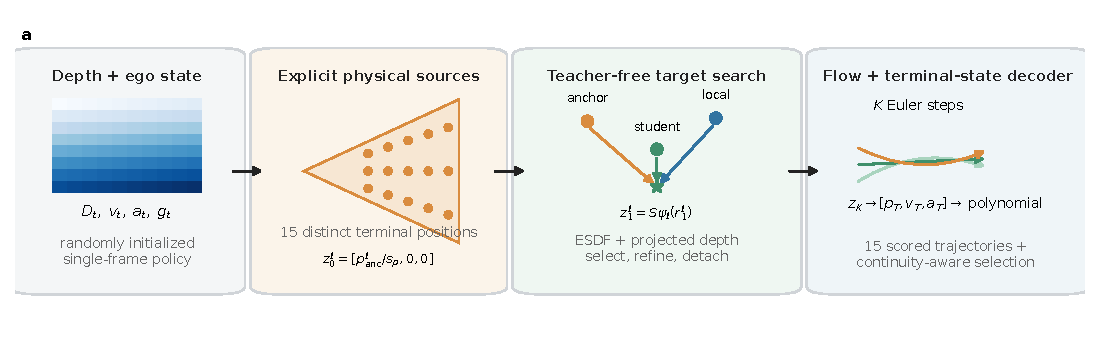
\includegraphics[width=\textwidth]{figures/fig1_method.pdf}
    \caption{LatticeFlow training and inference. Fifteen physical terminal-state anchors form deterministic source hypotheses. During training only, anchors, detached student predictions, and local perturbations are evaluated and monotonically refined by privileged trajectory costs. The conditional flow transports each anchor to a refined terminal state, which is decoded into a fifth-order polynomial and scored for selection.}
    \label{fig:method}
\end{figure*}

\subsection{Problem and Physical Lattice Source}

At planning time $t$, the policy receives a normalized depth image $D_t\in\mathbb{R}^{1\times96\times160}$ and body-frame state
\begin{equation}
    s_t=[v_t,a_t,g_t]\in\mathbb{R}^{9},
\end{equation}
where $v_t$, $a_t$, and $g_t$ are velocity, acceleration, and goal direction. No map, point cloud, distance field, previous image, or previous action enters the neural policy at deployment.

Inspired by the spherical motion-primitive construction of YOPO~\cite{lu2024yopo}, we use a $3\times5$ camera-aligned lattice with $L=15$ cells. A normalized primitive residual
\begin{equation}
 r^\ell=[\Delta\theta,\Delta\phi,\Delta r,
 \tilde v_T^\top,\tilde a_T^\top]^\top\in[-1,1]^9
\end{equation}
is mapped by a differentiable cell transform $\psi_\ell$ to body-frame terminal state $[p_T,v_T,a_T]$. This terminal state and the current state uniquely define a fifth-order polynomial over a fixed horizon.

Our flow operates in normalized physical coordinates
\begin{equation}
 z^\ell=S\psi_\ell(r^\ell)=
 [p_T^\top/s_p,v_T^\top/s_v,a_T^\top/s_a]^\top,
 \label{eq:physical-state}
\end{equation}
with $s_p=10$~m and $s_v=s_a=6\sqrt{3}$. Let $p_{\rm anc}^\ell$ be the position decoded at $r^\ell=0$. The source is
\begin{equation}
 z_0^\ell=[(p_{\rm anc}^\ell)^\top/s_p,0,0]^\top.
 \label{eq:source}
\end{equation}
Consequently, the 15 ODE states differ physically before any learned update. After integration, $z_K^\ell$ is mapped back through $r_K^\ell=\psi_\ell^{-1}(S^{-1}z_K^\ell)$ for trajectory reconstruction and control.

\subsection{Teacher-Free Cost-Refined Targets}

All neural weights, including the depth backbone, are randomly initialized. The last flow layer is initialized to zero, so the initial policy preserves Eq.~\eqref{eq:source}. For each cell, the current policy supplies a detached proposal $r_S^\ell$. We construct
\begin{equation}
 \mathcal C^\ell=\{0,\operatorname{sg}(r_S^\ell),
 \epsilon_{A,1},\ldots,\epsilon_{A,M_A},
 \operatorname{sg}(r_S^\ell)+\epsilon_{S,1},\ldots\},
 \label{eq:candidates}
\end{equation}
where $0$ decodes to the physical anchor, $\operatorname{sg}$ denotes stop-gradient, and the clipped Gaussian perturbations are used only for training-time exploration. Candidates are ranked independently per cell by
\begin{equation}
 J=J_{\rm smooth}+J_{\rm acc}+J_{\rm obs}+J_{\rm goal}
   +\lambda_dJ_{\rm depth}.
 \label{eq:cost}
\end{equation}
$J_{\rm obs}$ queries a map-derived Euclidean signed distance field (ESDF). For body-frame polynomial samples transformed into the depth-camera frame, the image term uses
\begin{align}
 u_n&=c_x-f_xy_n/x_n, & v_n&=c_y-f_yz_n/x_n,\\
 c_{d,n}&=d_{\max}D_t(u_n,v_n)-x_n,\\
 \rho(c)&=\beta\log\!\left(1+e^{(d_s-c)/\beta}\right),\\
 J_{\rm depth}&=N_v^{-1}\!\sum_{n\in\mathcal V}\rho(c_{d,n}).
\end{align}

Starting from the minimum-cost candidate $\bar r^\ell$, we propose normalized cost-gradient steps
\begin{equation}
 r^{\ell,+}=\operatorname{clip}\!\left(\bar r^\ell-\eta
 \frac{\nabla_{\bar r^\ell}\log(1+J)}
 {\operatorname{RMS}_{c}(\nabla_{\bar r^\ell}\log(1+J))+\varepsilon}\right).
 \label{eq:refine}
\end{equation}
A proposal replaces the current target only when its uncompressed trajectory cost decreases. The final target is detached and converted to $z_1^\ell=S\psi_\ell(r_1^\ell)$. Maps and ESDFs therefore supervise policy improvement but are absent at inference.

\subsection{Conditional Flow and Training Objective}

A convolutional depth backbone produces a $3\times5$ feature map. Velocity, acceleration, and goal are normalized and expressed in each primitive frame. A shared pointwise MLP conditions on the cell feature, transformed state, current physical flow state, sinusoidal time embedding, and learned lattice embedding:
\begin{equation}
 v_\theta^\ell=v_\theta(z_\tau^\ell,\tau,D_t,s_t,e_\ell).
\end{equation}
For $\tau\sim\mathcal U(0,1)$, the straight conditional path and target velocity are
\begin{align}
 z_\tau^\ell&=(1-\tau)z_0^\ell+\tau z_1^\ell,\\
 u_\tau^\ell&=z_1^\ell-z_0^\ell,
\end{align}
and
\begin{equation}
 \mathcal L_{\rm FM}=\mathbb E_{\tau,\ell}
 \lVert v_\theta^\ell-u_\tau^\ell\rVert_2^2.
 \label{eq:fm}
\end{equation}
Euler integration uses $K$ neural-function evaluations (NFE). A second head predicts the log-compressed trajectory cost of each integrated endpoint. The complete loss is
\begin{align}
 \mathcal L={}&\lambda_f\mathcal L_{\rm FM}+\lambda_e\mathcal L_{\rm end}
 +\lambda_J\log(1+J)+\lambda_s\mathcal L_{\rm score}\nonumber\\
 &+\lambda_c\mathcal L_{\rm cons}+\lambda_l\mathcal L_{\rm lat}.
 \label{eq:total-loss}
\end{align}
$\mathcal L_{\rm cons}$ applies Huber consistency to endpoints and centered scores under small depth/state perturbations. $\mathcal L_{\rm lat}$ penalizes horizontal and vertical second differences across neighboring cells. These terms encourage local robustness; they are not temporal supervision because training samples are independent.

The source-noise variance is zero. Thus a fixed input deterministically produces one trajectory per cell, and the 15 cells carry the avoidance alternatives. This structured flow does not itself guarantee that the minimum-score cell remains unchanged over time.

\subsection{Optional Continuity-Aware Selection}

For deployments that favor command continuity, a one-step selector stores the previously selected endpoint $p_{t-1}^{*}$ and adjusts each current score:
\begin{equation}
 \hat q_t^\ell=q_t^\ell+\lambda_p\lVert p_t^\ell-p_{t-1}^{*}\rVert_2.
\end{equation}
The previous cell is retained while its raw score is within margin $\delta_q$ of the current raw minimum; otherwise the minimum adjusted score is selected. This state is outside the neural policy and is ablated separately. The real flights reported below use raw selection with this selector disabled.
